\documentclass[12pt,a4paper]{article}

\usepackage[brazil]{babel}
\usepackage{fontspec}
\usepackage{xeCJK}
\usepackage{xcolor}
\usepackage{ruby}
\usepackage{amsmath}
\usepackage{tcolorbox}
\usepackage{enumitem}
\usepackage{tabularx}
\usepackage{booktabs}

\setmainfont{Latin Modern Roman}
\setCJKmainfont{Noto Serif CJK JP}

\definecolor{jpnavy}{RGB}{20,35,60}
\definecolor{jpred}{RGB}{180,40,40}
\definecolor{lighthight}{RGB}{245,247,250}
\definecolor{jppurple}{RGB}{110, 70, 120}

\pagestyle{empty}

\begin{document}

\begin{center}
    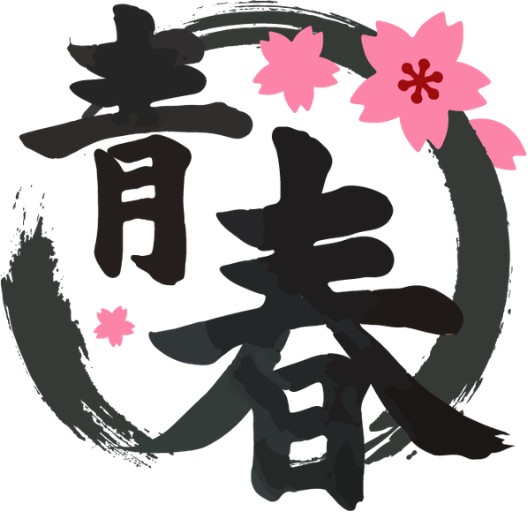
\includegraphics[height=2cm, keepaspectratio]{../Seishun.png}\\
    \vspace{0.3cm}
    {\LARGE\bfseries 第二課}\\[4pt]
\end{center}

\vspace{0.3cm}
\hrule height 1pt
\vspace{0.5cm}

\begin{tcolorbox}[colback=jppurple!6, colframe=jppurple, title=\textbf{Dica Cultural}, fonttitle=\bfseries]
\small
No Japão, o uso de máscaras faciais (\textit{masuku}) é um hábito cultural consolidado de respeito ao próximo para evitar a contaminação. Ao ir ao hospital ou farmácia, é essencial apresentar o \textbf{Hokenshou} (Cartão do Seguro de Saúde). 
\end{tcolorbox}

\vspace{0.2cm}

\subsection*{Sistemas de Contagem e Sufixos}

\vspace{0.2cm}


\begin{tabularx}{\textwidth}{c X X}
\toprule
\textbf{Nº} & \textbf{Japonês (Kanji / Kana)} & \textbf{Leitura (Romaji)} \\
\midrule
1 & 一 (いち) & ichi \\
2 & 二 (に) & ni \\
3 & 三 (さん) & san \\
4 & 四 (よん / し) & yon / shi \\
5 & 五 (ご) & go \\
6 & 六 (ろく) & roku \\
7 & 七 (なな / しち) & nana / shichi \\
8 & 八 (はち) & hachi \\
9 & 九 (きゅう / く) & kyū / ku \\
10 & 十 (じゅう) & jū \\
\bottomrule
\end{tabularx}


\textbf{Perguntando a Temperatura (Febre)}
\begin{itemize}[leftmargin=*]
    \item \textbf{度 (ど / do):} Sufixo para "graus".
    \item \textbf{何度ありますか？ (\textit{Nan do arimasu ka?}):} Quantos graus você tem? / Qual é a sua temperatura?
\end{itemize}

\vspace{0.3cm}

\textbf{Perguntando e Respondendo a Idade}
\begin{itemize}[leftmargin=*]
    \item \textbf{歳(さい / sai):} Sufixo para idade.
    \item \textbf{何歳ですか？ (\textit{Nansai desu ka?}):} Quantos anos você tem? (Padrão)
    \item \textbf{おいくつですか？ (\textit{O-ikutsu desu ka?}):} Quantos anos você tem? (Forma polida / Respeitosa)
\end{itemize}

\vspace{0.2cm}

\textbf{Exceções de Pronúncia na Contagem de Idade (歳 / \textit{sai}):}

\noindent
\begin{tabularx}{\textwidth}{l X X}
\toprule
\textbf{Idade} & \textbf{Escrita (Kanji)} & \textbf{Leitura (Romaji)} \\
\midrule
1 ano & 一歳 & Issai \\
8 anos & 八歳 & Hassai \\
10 anos & 十歳 & Jussai / Jissai \\
20 anos & 二十歳  & Hatachi \textit{(Não usa o sufixo sai)} \\
\bottomrule
\end{tabularx}




\vspace{0.4cm}

\textbf{Exercício 1: Prática de Números}

\small
\textbf{A. Complete com numeros:}
\begin{enumerate}[label=\arabic*.]
    \item Yon Jū = \underline{40}
    \item Jū go = \underline{15} 
    \item Nana = \underline{7}
    \item Jū = \underline{10} 
    \item Shichi = \underline{7} 
    \item Roku = \underline{6} 
    \item Hachi = \underline{8} 
    \item Ichi = \underline{1} 
    \item San = \underline{3} 
\end{enumerate}

\textbf{B. Escreva a idade em japones:} 
\begin{enumerate}[label=\arabic*.]
    \item 3 anos = \underline{Sansai (三歳)} 
    \item 2 anos = \underline{Nisai (二歳)} 
    \item 1 ano = \underline{Issai (一歳)} 
    \item 20 anos = \underline{Hatachi (二十歳)} 
\end{enumerate}

\newpage
\subsection*{Vocabulário: Partes do Corpo e Saúde}

\vspace{0.2cm}


\begin{tabularx}{\textwidth}{l X X}
\toprule
Palavra (Romaji) & Kanji / Kana & Tradução em Português \\
\midrule
Atama & 頭 (あたま) & Cabeça \\
Me / Mimi / Hana & 目 / 耳 / 鼻 & Olho / Orelha / Nariz \\
Onaka & お腹 (おなか) & Barriga / Estômago \\
Nodo & 喉 (のど) & Garganta \\
Itai & 痛い (いたい) & Dolorido / Sentir dor \\
Netsu & 熱 (ねつ) & Febre \\
Kaze & 風邪 (かぜ) & Resfriado / Gripe \\
Kusuri & 薬 (くすり) & Remédio \\
\bottomrule
\end{tabularx}
元気？ (\textit{Genki?}) 
お元気ですか？ (\textit{O-genki desu ka?})

\vspace{0.4cm}

\textbf{ Associação de Vocabulário}

\small
Relacione a coluna da esquerda (Japonês/Romaji) com o seu significado em português na coluna da direita:

\vspace{0.2cm}


\begin{tabularx}{\textwidth}{l X c X}
( 1 ) & Netsu (熱) & ( 2 ) & Remédio \\
( 2 ) & Kusuri (薬) & ( 3 ) & Dor / Dolorido \\
( 3 ) & Itai (痛い) & ( 1 ) & Febre \\
( 4 ) & Atama (頭) & ( 5 ) & Barriga / Estômago \\
( 5 ) & Onaka (お腹) & ( 4 ) & Cabeça \\
( 6 ) & Hokenshou (保険証) & ( 6 ) & Cartão de Seguro de Saúde \\
\end{tabularx}



\vspace{0.6cm}

\begin{center}
    {\LARGE\bfseries 会話 (Diálogo no Hospital)}
\end{center}

\textit{Cenário: Tanaka não está se sentindo bem e vai à consulta médica com o Dr. Yamada.}

\vspace{0.8em}

\textbf{\ruby{医師}{いし}:} 田中さん、こんにちは。どうしましたか？\\
\textit{Ishi:} Tanaka-san, konnichiwa. Dou shimashita ka?\\
Médico: \underline{Tanaka-san, olá. Como você está se sentindo?} 

\vspace{0.4em}

\textbf{\ruby{田中}{たなか}:} 頭と体が痛いです。\\
\textit{Tanaka:}  atama to karada ga itai desu.\\
Tanaka: \underline{Minha cabeça e meu corpo estão doendo.} 

\vspace{0.4em}

\textbf{\ruby{医師}{いし}:} 熱はありますか？\\
\textit{Ishi:} Netsu wa arimasu ka?\\
Médico: \underline{Você tem febre?} 

\vspace{0.4em}

\textbf{\ruby{田中}{たなか}:} はい、38度あります。少し咳も出ます。\\
\textit{Tanaka:} Hai, san-jū-hachi do arimasu. Sukoshi seki mo demasu.\\
Tanaka: \underline{Sim, estou com 38 graus. Também estou com um pouco de tosse.} 

\vspace{0.4em}

\textbf{\ruby{医師}{いし}:} 風邪ですね。薬を二つ出しておきます。一日三回飲んでください。\\
\textit{Ishi:} Kaze desu ne. Kusuri wo futatsu dashite okimasu. Ichi-nichi san-kai nonde kudasai.\\
Médico: \underline{É um resfriado. Vou receitar dois remédios. Tome três vezes ao dia, por favor.} 

\vspace{0.4em}

\textbf{\ruby{田中}{たなか}:} わかりました。ありがとうございます。\\
\textit{Tanaka:} Wakarimashita. Arigatou gozaimasu.\\
Tanaka: \underline{Entendi. Muito obrigado(a).} 

\vspace{0.4em}

\textbf{\ruby{医師}{いし}:} お大事にどうぞ。\\
\textit{Ishi:} O-daiji ni douzo.\\
Médico: \underline{Melhoras! / Cuide-se.} 

\newpage

\vspace{0.5cm}

\begin{tcolorbox}[colback=jppurple!6, colframe=jppurple, title=\textbf{Dinâmica em Grupo (Simulação de Consulta)}, fonttitle=\bfseries]
\small
Em duplas (1 Médico, 1 Paciente), pratiquem uma consulta rápida:
\begin{enumerate}[leftmargin=*]
    \item \textbf{Sintomas:} O paciente explica onde sente dor usando a estrutura \textit{"[Parte do corpo] ga itai desu"}.
    \item \textbf{Diagnóstico:} O médico orienta o paciente a tomar o remédio usando os contadores (\textit{ex: Kusuri wo futatsu nonde kudasai}).
    \item \textbf{Despedida:} Finalizem a consulta com a expressão \textit{"O-daiji ni"}.
\end{enumerate}
\end{tcolorbox}

\vspace{0.4cm}

\begin{center}
    \small\color{gray} \textit{お疲れ様でした！(Otsukaresama deshita!)}
\end{center}

\end{document}